\documentclass[12pt]{article}%
\usepackage{amsfonts}
\usepackage{fancyhdr}
\usepackage{comment}
\usepackage[letterpaper, top=2.5cm, bottom=2.5cm, left=2.2cm, right=2.2cm]%
{geometry}
\usepackage{times}
\usepackage{changepage}
\usepackage{multirow}
\usepackage{amssymb}
\usepackage{amsmath}
\usepackage{tikz}
\usetikzlibrary{arrows.meta}
\usepackage{graphicx}%
\graphicspath{ {images/} }
\usepackage{amsmath}
\setcounter{MaxMatrixCols}{30}
\newtheorem{theorem}{Theorem}
\newtheorem{acknowledgement}[theorem]{Acknowledgement}
\newtheorem{algorithm}[theorem]{Algorithm}
\newtheorem{axiom}{Axiom}
\newtheorem{case}[theorem]{Case}
\newtheorem{claim}[theorem]{Claim}
\newtheorem{conclusion}[theorem]{Conclusion}
\newtheorem{condition}[theorem]{Condition}
\newtheorem{conjecture}[theorem]{Conjecture}
\newtheorem{corollary}[theorem]{Corollary}
\newtheorem{criterion}[theorem]{Criterion}
\newtheorem{definition}[theorem]{Definition}
\newtheorem{example}[theorem]{Example}
\newtheorem{exercise}[theorem]{Exercise}
\newtheorem{lemma}[theorem]{Lemma}
\newtheorem{notation}[theorem]{Notation}
\newtheorem{problem}[theorem]{Problem}
\newtheorem{proposition}[theorem]{Proposition}
\newtheorem{remark}[theorem]{Remark}
\newtheorem{solution}[theorem]{Solution}
\newtheorem{summary}[theorem]{Summary}
\newenvironment{proof}[1][Proof]{\textbf{#1.} }{\ \rule{0.5em}{0.5em}}

\newcommand{\Q}{\mathbb{Q}}
\newcommand{\R}{\mathbb{R}}
\newcommand{\C}{\mathbb{C}}
\newcommand{\Z}{\mathbb{Z}}

\newcommand*{\pd}[3][]{\ensuremath{\frac{\partial^{#1} #2}{\partial #3}}}

\usepackage{enumerate}% http://ctan.org/pkg/enumerate
\usepackage{array}% http://ctan.org/pkg/array
\newcolumntype{M}{>{$}c<{$}}


\begin{document}

\title{CS 440/ECE448 Homework 7}
\author{Tanishq Dubey (tdubey3)}
\date{\today}
\maketitle
\section*{Problem 1}
    \begin{enumerate}[a)]
        \item \textbf{AND} \\
        The weights should be equal for all three inputs, thus $w_1$, $w_2$, $w_3$, are all equal to $0.33$. In order for this function to only activate when all inputs are active, we must adjust the bias so that this behavior occurs. This means that the bias, $b$ must be -1 because when all inputs are on, our inputs add up to $0.33 + 0.33 + 0.33 = 1$.
        \item \textbf{OR} \\
        Again, the weights for our inputs should be equal, thus $w_1$, $w_2$, $w_3$, are all equal to $0.33$. In this situation, however, we are not looking for all inputs to be enabled, but any the one inputs to be enabled. Thus our bias, $b$, for this situation is $-.33$. With this, when any input is activated, our system is activated as $-.33 + .33 = 0$
        \item \textbf{At most two} \\
        For this system, we can have 0 inputs, 1 input, or two inputs simultaneously enabled, but 3 inputs should result in the system being off. For this then, our weights must be, again, equal, but in the negative direction. This means that our weights, $w_1$, $w_2$, and $w_3$ are all equal to $-0.33$. With this then, we can set our bias, $b$ to $0.66$. This means that our system will only be disabled when three inputs are on because $3(-0.33) + 0.66 = -0.33$
        \item \textbf{2 out-of 3} \\
        This system cannot be implemented as there is no bias and weight combination that allows for this. We can come incredibly close, as with our "At most two" system, however, with our current problem, we cannot account for the 0-input state. Because of this there is no solution for this.
    \end{enumerate}

\section*{Problem 2}
    \begin{enumerate}[a)]
        \item A circle around the origin has a VC dimension of 1, because at a minimum, it can shatter a singular point that is either within the circle or external to the circle.
        \item A circle that can be arbitrarily be positioned in a 2D plane has a VC dimension of 2. This is The minimum because it is clear to see that two points can easily be classified by moving the circle to a arbitrary center point.
    \end{enumerate}
    

\section*{Problem 3}
    \begin{enumerate}[a)]
        \item 4
        \item This number was chosen after running the neural net on training data for 75,000 runs on various numbers of neurons in the hidden layer. Appendix A displays the various errors of a set number of runs for varying numbers of neurons, specifically, 2, 4, and 50 hidden layer neurons. Of these tests, 4 showed a clear learning curve with the least amount of noise, hence it was chosen.
        \item Error on the training set was $0.0\%$
        \item Error on the testing set was $0.3857\%$
        \item No division
        \item To stop updating weights, the past 100 errors should have been within $2\%$ of each other.
        \item My $\alpha = 0.2$
        \item 10,572
        \item Refer to Appendix A
    \end{enumerate}
    
\newpage
\section*{Appendix A}
    \textbf{2 Nodes over 75000 Runs}\\
    \begin{center}
        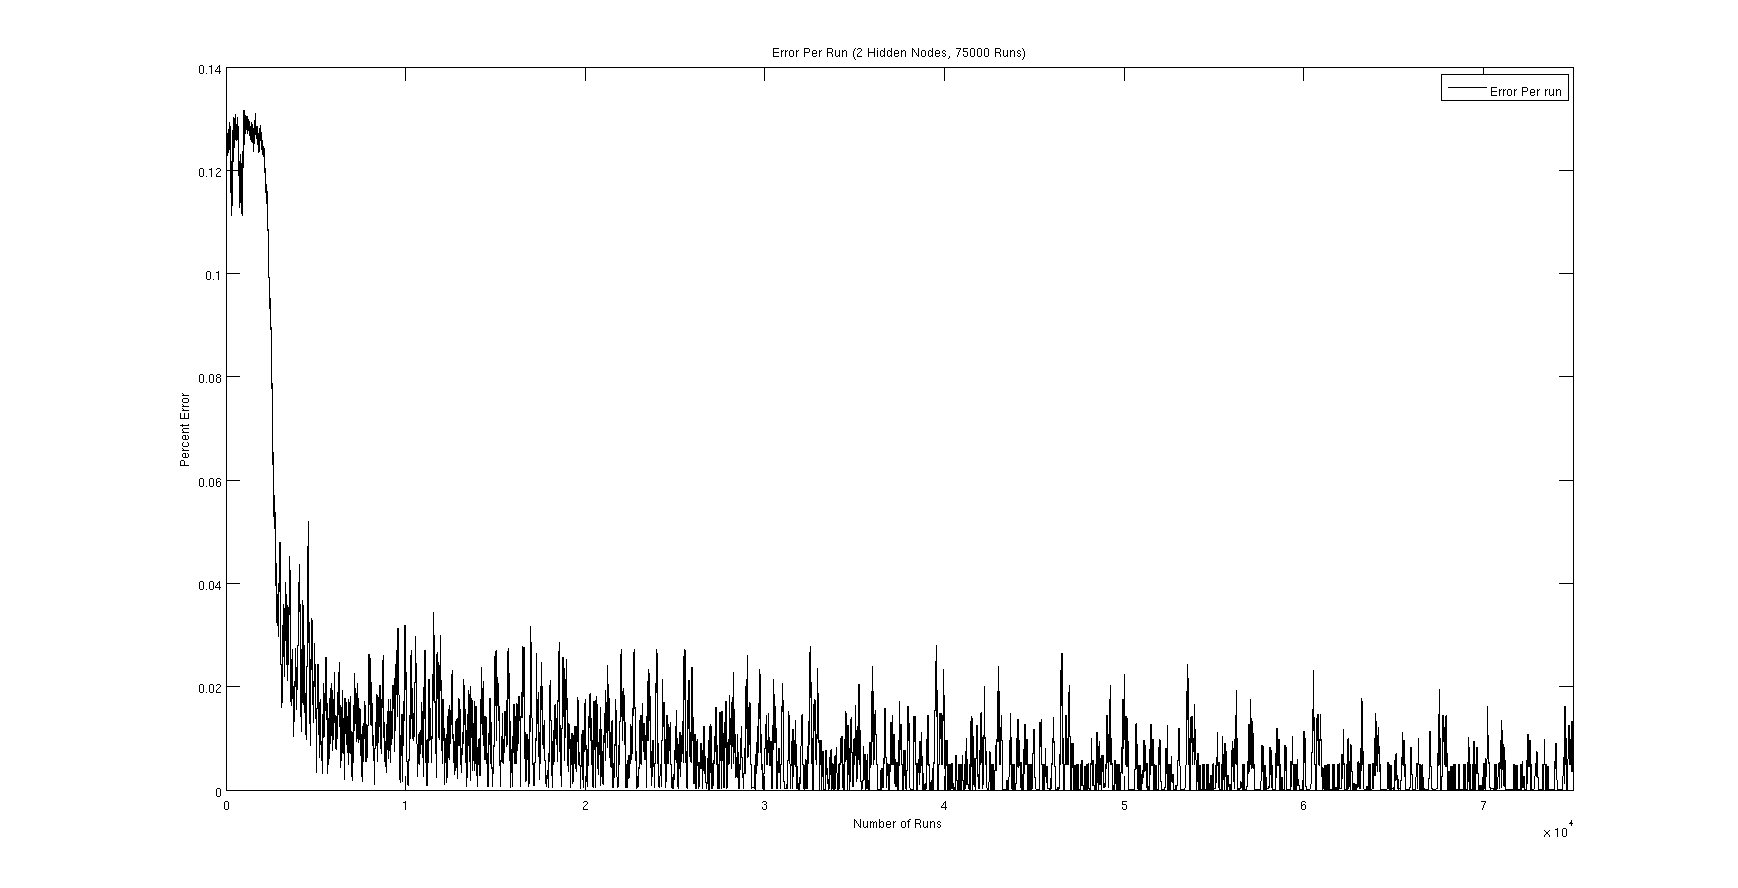
\includegraphics[scale=.3]{2node75000}\\
    \end{center}
    \textbf{4 Nodes over 75000 Runs}\\
    \begin{center}
        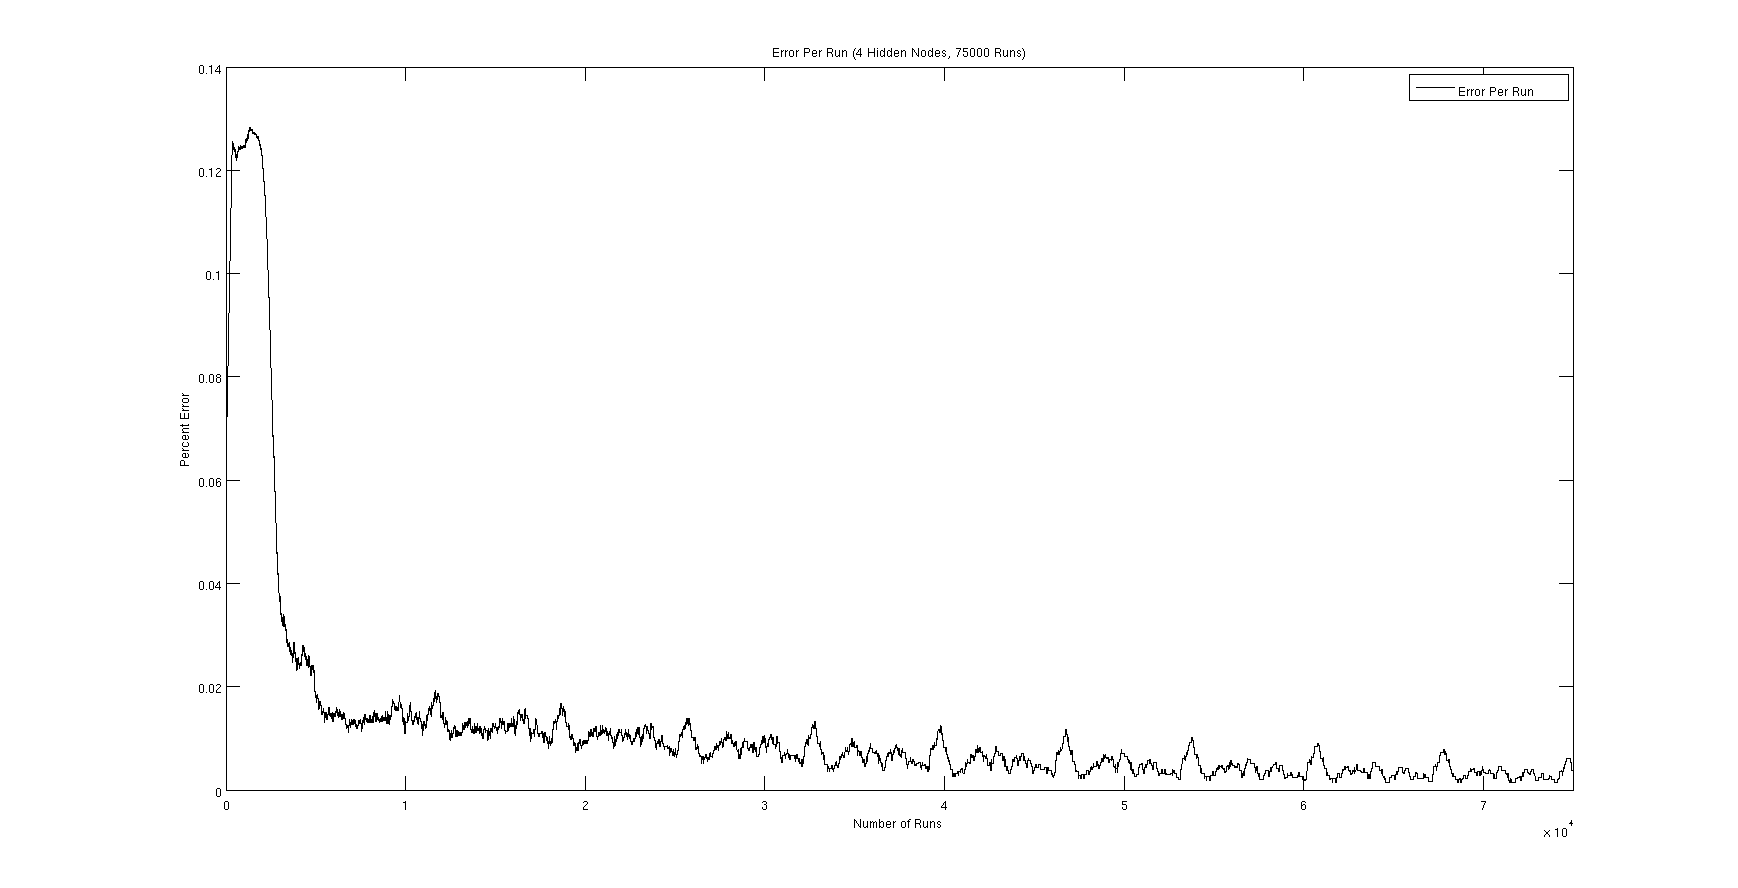
\includegraphics[scale=.3]{4node75000}\\
    \end{center}
    \newpage
    \textbf{50 Nodes over 75000 Runs}\\
    \begin{center}
        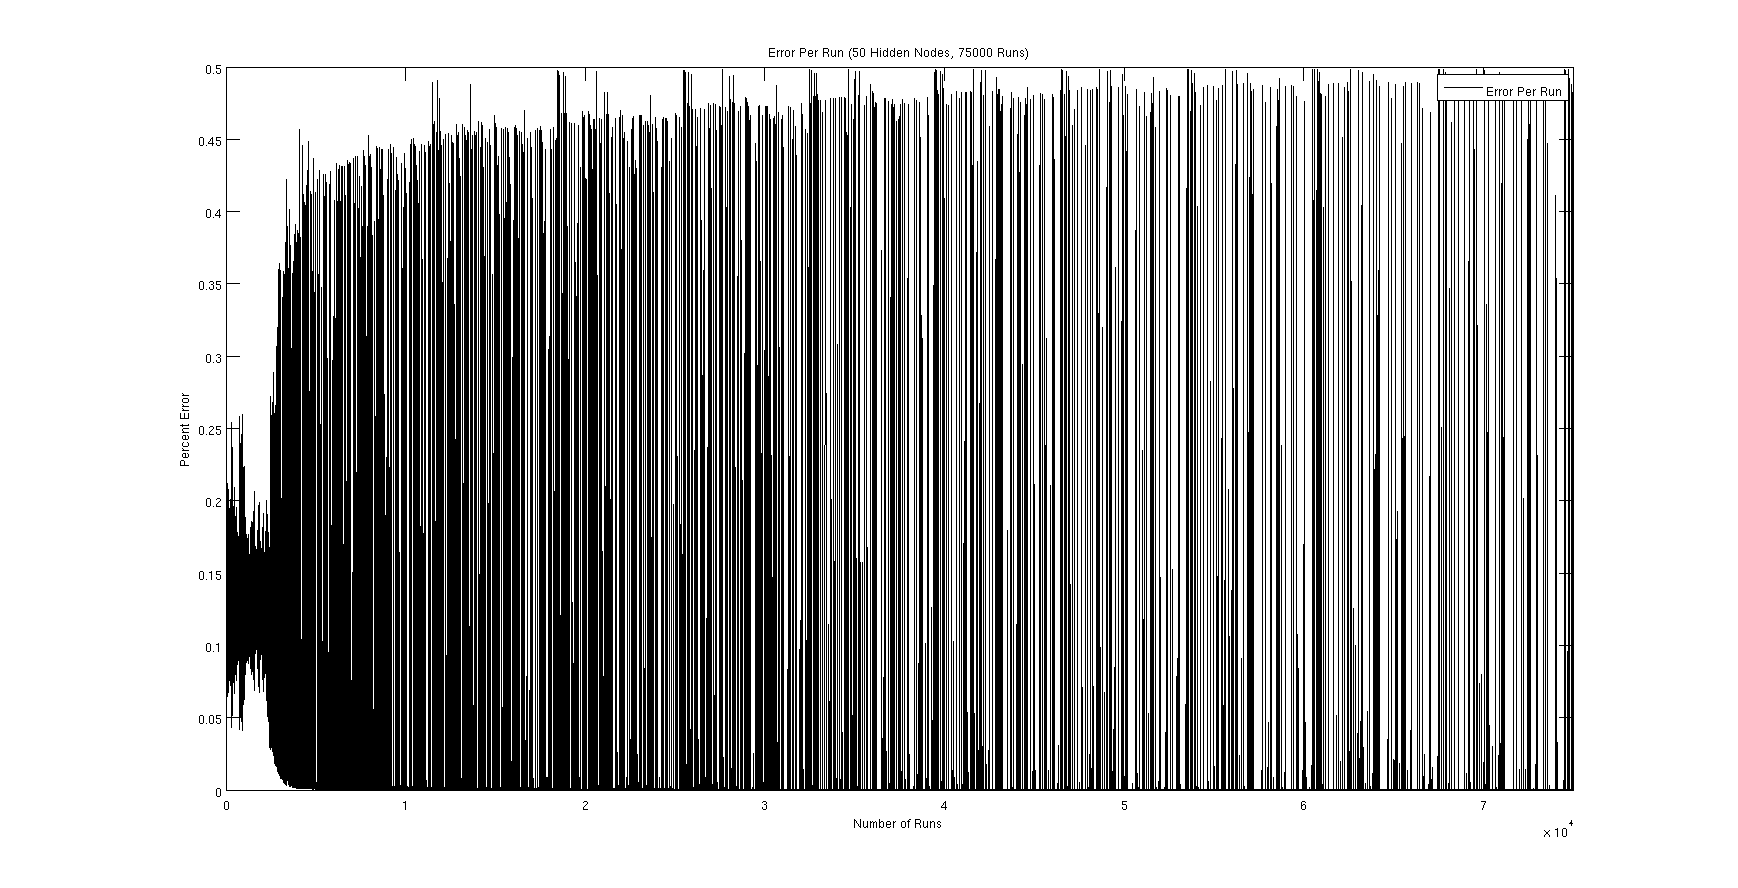
\includegraphics[scale=.3]{50node75000}\\
    \end{center}

    
\end{document}